\chapter{Conceptual Design Work}
\label{chap:conceptual-design-work}

\section{Overview}
\label{sec:conceptual-overview}

In this chapter we present our approach to the problem defined in \Cref{sec:problem-definition}, while justifying any design decisions made at any particular stage. At first, we clearly describe the input and output of the system. Then, we provide an overview of our approach, before explaining each step and decision separately.


\section{Input and Output of the System}
\label{sec:input-output}

In contrast to the majority of the systems that perform API usage mining, where the input of the system is usually a repository of source code files, as well as a class or a method of the target API, our system needs a slightly different input as this is described below:

\begin{description}
\item[Input] A repository of Java source code files (client code), as well as a \texttt{.arff} file, consisting of client methods, and of their associated API call sequences. Each row in the \texttt{.arff} file is in the form presented in \Cref{listings:arff-transaction}, where the \texttt{client\_method} (also called ``caller'') and any \texttt{API\_call\textsubscript{i}} (also called ``call'') are fully qualified names. A sample row in the \texttt{.arff} file for the \texttt{Twitter4J} API is shown in \Cref{listings:twitter4j-arff-transaction}.
\item[Output] A ranked list of Java snippets. An example is shown in \Cref{listings:exp3-hdbscan-top-snippets}.
\end{description}

\begin{figure}[h]
  \lstinputlisting[language=arff]{listings/ArffTransaction.arff}
  \vspace{-10pt}
  \caption[Transaction in the \texttt{.arff} file]{General form of a transaction in a \texttt{.arff} file.}
\label{listings:arff-transaction}
\end{figure}

\begin{figure}[h]
  \lstinputlisting[language=arff]{listings/Twitter4jArffTransaction.arff}
  \vspace{-10pt}
  \caption[Transaction in the \texttt{twitter4j.arff} file]{Transaction in the \texttt{twitter4j.arff} file.}
\label{listings:twitter4j-arff-transaction}
\end{figure}

As revealed by the input of our system, we aim to mine usage example for the entire target API, rather than for a single method or a class of it. However, an input in the latter forms would only involve filtering of the mined snippets.


\subsection{Justifying the Form of the Input}
\label{subsec:input-form}

Our decision to use a different input from that used in the literature, stems from the fact that our team has already created a well-formed local corpus of the top Java projects in GitHub\footnote{\url{http://groups.inf.ed.ac.uk/cup/javaGithub/}} \cite{Allamanis:2013}. This, at first, prompted us to use this corpus as the source of our system. 

Furthermore, taking into account the limited time for the elaboration of this dissertation, and the fact that there has already been some previous work on API usage mining from our team in \cite{Fowkes2:2015}, we decided to use the \textsc{Example} dataset presented in that work. This would allow us to spent more valuable time on the main task of mining patterns, rather than on that of finding relevant files in the GitHub Java corpus. This dataset includes popular libraries and frameworks that also contain an \texttt{examples} directory, which is moreover going to enable the comparison of our system's mined snippets with these handwritten examples. For each library, \nolink{\citeauthor{Fowkes2:2015}} have created a directory of source code files that import a class belonging a (sub)package of the library (client code), while they have also generated the aforementioned \texttt{.arff} files\footnote{The best-effort approach used to extract the API call sequences, and to generate the \texttt{.arff} file subsequently, is described extensively in \cite{Fowkes2:2015}, and is out of the scope of this dissertation.}.

We point out that, ideally, there would exist a mapping between the \texttt{.arff} transactions and their associated source code files. However, as this information was not available for the \textsc{Example} dataset, we created a script that uses a best-effort approach, in order to do this. Our approach uses the fully qualified name of each client method, with the aim of finding its source code file. When there are duplicate class files, (these are labelled: \texttt{Class.java}, \texttt{Class\_2.java}, \texttt{Class\_3.java}, etc), we parse the package declaration of each class file, and match it to that of the client method's one.


\section{Overview of the Proposed Methodology}
\label{sec:methodology-overview}

Our methodology may be summarised in the following points:

\newcommand\litem[1]{\item{\bfseries #1\\}}
\begin{enumerate}
\litem{Clean the \texttt{.arff} file} This step filters the \texttt{.arff} file, by removing any sequences that are not of interest, as we are going to explain in \Cref{sec:data-preprocessing}.
\litem{Cluster the sequences in the cleaned \texttt{.arff} file} In this step, we leverage clustering techniques, in order to cluster the API call sequences in the \texttt{.arff} file. We analyse the process in \Cref{sec:clustering-step}.
\litem{Select a fixed number of sequences from each cluster} This is a clustering postprocessing step, that selects the top sequences from each cluster, as briefly explained in \Cref{sec:sequence-selection}.
\litem{Generate a summarised snippet for the source code associated with each selected sequence} In this step we retrieve the source code files that are associated with the sequences that have been selected in the previous step, and generate a summarised snippet for each of them, by leveraging a summarisation algorithm we implemented. We explain the process followed, as well as the decision to implement our own summarisation algorithm, in \Cref{sec:snippet-generation}. 
\litem{Select a single summarised snippet from each cluster} In this step we use a tree edit distance metric, in order to select a single snippet from each cluster, as explained in \Cref{sec:select-snippet}.
\litem{Rank the selected snippets, based on their support} This is the final step, where we rank the snippets in order of decreasing support. This is described in \Cref{sec:results-presentation}.
\end{enumerate}


\section{Cleaning the \texttt{.arff} File}
\label{sec:data-preprocessing}

A crucial step that precedes the application of clustering techniques to the data is the preprocessing step, which basically refers to the appropriate cleaning, that aims to remove the data that could break down even a powerful clustering algorithm. However, data cleaning has not only to do with the clustering quality; it also refers to the removal of any data that is not of interest. In our case, we proceed to the following removals:

\begin{itemize}
\litem{Remove callers that refer to different versions of the same source code file} An identical caller name indicates a different version of the same file. We remove multiple versions of the same source code file, as we noticed that most of them are identical in terms of API call sequences, and that they would affect the clustering process. An example is shown in \Cref{listings:versions}.
\litem{Remove singleton sequences} These are the sequences that contain only a single API call. We claim that singletons do not contain any useful information, as they do not show any interaction between different API methods. An example is shown in \Cref{listings:singleton}.
\litem{Remove pseudo-singleton sequences} These are the sequences that contain only a single API method, which is invoked multiple times. An example is shown in \Cref{listings:identical}.
\litem{Removes unique\footnote{We define a \textit{unique sequence} as this sequence for which there is no other sequence that contains the same API calls, invoked in the same order. That is, there is no other identical sequence.} sequences, if specified so} An interesting decision here is that of whether to remove the sequences that are unique. Although the removal of the unique sequences would result to more tight clusters, we would probably miss rare patterns, while the fact that they are unique does not mean that they do not share API calls with other sequences. Based on this, we decided to have this feature as a parameter of the preprocessing step, and consider this on the evaluation of the system.
\end{itemize}

\begin{figure}[ht]
\lstinputlisting[language=arff]{listings/Versions.arff}
\vspace{-10pt}
\caption[Example indicating multiple versions of the same source code file]{Example indicating multiple versions of the same source code file.}
\label{listings:versions}
\vspace{-5pt}
\end{figure}

\begin{figure}[ht]
\vspace{-10pt}
\lstinputlisting[language=arff]{listings/Singleton.arff}
\vspace{-10pt}
\caption[Example indicating a singleton sequence]{Example indicating a singleton sequence.}
\label{listings:singleton}
\vspace{-5pt}
\end{figure}

\begin{figure}[ht]
\vspace{-10pt}
\lstinputlisting[language=arff]{listings/Identical.arff}
\vspace{-10pt}
\caption[Example indicating a pseudo-singleton sequence]{Example indicating a pseudo-singleton sequence.}
\label{listings:identical}
\vspace{-5pt}
\end{figure}


\section{Clustering the Sequences}
\label{sec:clustering-step}

In this section we analyse any design decisions that are related to the clustering process. For instance, we justify our decision to apply clustering techniques at this stage, as well as our decision to cluster the sequences using a distance matrix instead of a feature vector. In addition to that, we visualise the \texttt{Twitter4J} dataset, in order to investigate whether there is a clear notion of clusters. Finally, we provide a brief overview of the clustering techniques we implemented, which are going to be analysed extensively in the next chapter.


\subsection{Why Clustering at This Stage?}
\label{subsec:clustering-decision}

Our decision to use clustering techniques, and more specifically at this stage, is quite simple. At first, looking at the client code in \Cref{listings:cluster-snippet1,listings:cluster-snippet2}, we see that these two snippets are quite similar, while they contain the same API calls (these are highlighted appropriately). A clustering technique that is based on the API call sequences of the client code would cluster these two snippets together. Taking into account the large number of files in the repository, this seems a more efficient approach than a clustering technique that would consider the structure of the client code, too. After all, we take into consideration the structure of the clustered snippets at a next stage, as described in \Cref{sec:select-snippet}. Hence, this approach is a balance between time overhead and quality improvement.

\begin{figure}[h]
\lstinputlisting[language=Java,style=Java]{listings/ClusterSnippet1.java}
\vspace{-10pt}
\caption[Sample client code 1]{Sample client code where the API calls are highlighted.}
\label{listings:cluster-snippet1}
\end{figure}

\vspace{-10pt}

\begin{figure}[H]
\lstinputlisting[language=Java,style=Java]{listings/ClusterSnippet2.java}
\vspace{-10pt}
\caption[Sample client code 2]{Sample client code that contains the same API calls with the client code presented in \Cref{listings:cluster-snippet1}.}
\label{listings:cluster-snippet2}
\end{figure}

\vspace{-20pt}

\subsection{Feature Vector vs Distance Matrix}
\label{subsec:feature-extraction}

The common input of a clustering algorithm is a feature vector that is generated from the data. While clustering using a feature vector has the advantage that one can apply almost every clustering technique on the vector, we identify a few problems here; one of them is that the designer should decide on the features to be used. In our case, a feature vector could be a boolean vector, where each future would represent a unique API method\footnote{Notice that we are talking about API methods and not about API calls; an API method may be called multiple times.}. As we understand, in this way we would represent the data as itemsets, rather than as sequences. The latter could be achieved by defining additional features that reveal the order in which the API methods are invoked.

Instead of generating a feature vector, probably the most common way to cluster sequences is to compute a distance/similarity matrix, using a sequence distance/similarity metric, and then cluster the sequences using this matrix. This approach cannot leverage algorithms that are based on Euclidean distances (such as the $k$-means one), but the majority of clustering techniques can be modified in order to receive a distance matrix instead of a feature vector as an input\footnote{We point out here that, while pre-computing a distance matrix would result to higher memory usage, it would also lead to lower computational/time complexity, as any clustering algorithm would compute this information at some point.}. In order to compute the similarity between any two sequences we tried several metrics, and we are going to analyse the most consistent of them in the next chapter. Our conclusion is that there is no significant difference in the results when using the one or the other, and thus we decided not to consider this as a parameter during the evaluation of the system.


\subsection{Visualising the Data}
\label{subsec:data-visualisation}

Considering that we now have a representation of our data, it would be interesting to try to visualise this. Taking into account the high-dimensional nature of the data, this would be tricky enough, though. Dimensionality reduction methods like the popular \textit{PCA} or the \textit{Isomap} kernels would not work in our case, as the data seem quite sparse. A technique that is usually applied in high-dimensional sparse data is this of the \textit{t-SNE} method \cite{Maaten:2008}, which converts similarities between data points to joint probabilities. Trying to visualise the data\footnote{At this step, we do not remove unique sequences in order to have a comprehensive picture of our data.} using the implementation of the t-SNE algorithm, which is part of Python's \texttt{scikit-learn} library\footnote{\url{http://scikit-learn.org/stable/modules/generated/sklearn.manifold.TSNE.html}}, we noticed that, although there were a few dense areas, most of the sequences are unique and similar to multiple other sequences, a fact that may confuse the t-SNE algorithm. A possible visualisation of the data is shown in \Cref{images:tsne-plot}. We should point out here that the visualisation is highly affected by several factors, such as the sequence similarity metric, and the parameters used in the t-SNE algorithm. In any case, this plot indicates that it is difficult enough to predict the number of clusters -even with the use of popular metrics such as the \textit{silhouette coefficient} or the \textit{Elbow} method as we ascertained later- as there are no clear, with respect to cohesion and even more to separation, clusters in the data.

\begin{figure}[h]
  \centering
  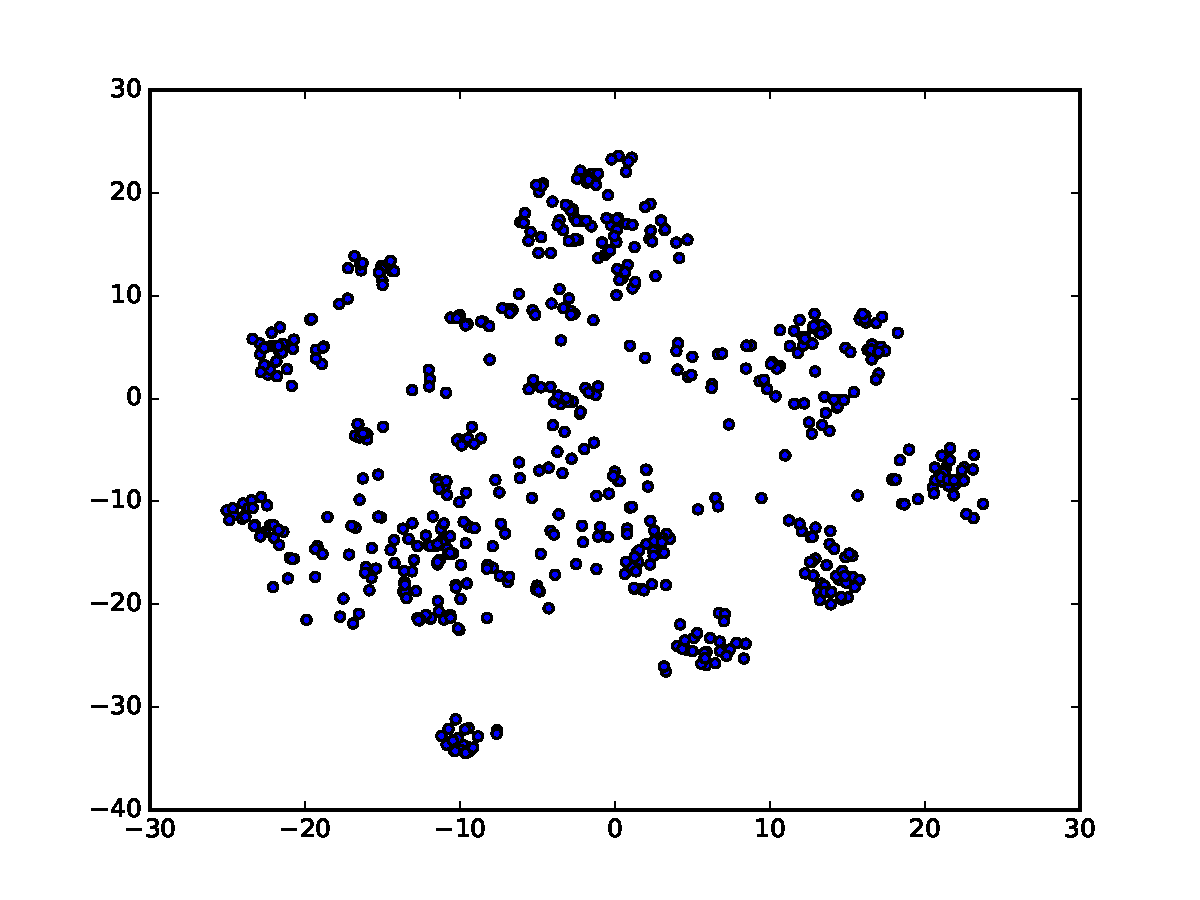
\includegraphics[scale=0.4]{images/tsne-plot}
  \caption[Plotting the data using the \textit{t-SNE} technique]{Plotting the sequences of the \texttt{Twitter4J} API using the \textit{t-SNE} algorithm.}
  \label{images:tsne-plot}
\end{figure}


\subsection{Applying Clustering Techniques}
\label{subsec:clustering-techniques}

Regarding the clustering techniques that have been investigated in the current project, although we tried several algorithms, two of them have been proven promising, and thus we decided to evaluate two different versions of the system, with respect to the clustering algorithm used. The first one uses an implementation of the $k$-medoids algorithm, the basic version of which has been described in \Cref{subsec:k-medoids}, while the second one is a hierarchical version of the DBSCAN algorithm (named \textit{HDBSCAN}, and introduced in \cite{Campello:2013}). We also tried different approaches for the initialisation of the medoids for the $k$-medoids technique, and implemented the $k$\verb!++! technique which has been proven more efficient than a random initialisation for this task. Regarding the number of clusters, we tried to predict them using popular methods, including the Elbow or the silhouette coefficient ones, however, none of them showed any cut-off point, and thus we decided to hard-code this parameter, using our intuition.

In any case, the result of the clustering process will be a clustered version of the \texttt{.arff} file. An example is shown in \Cref{listings:arff-clustering}, where the callers whose sequences have been clustered together are highlighted using the same colour.

\begin{figure}[h]
  \lstinputlisting[language=arff,style=arff]{listings/SequenceClustering.arff}
  \vspace{-10pt}
  \caption[Clustered \texttt{.arff} file]{Clustered version of the \texttt{.arff} file.}
\label{listings:arff-clustering}
\end{figure}


\section{Selecting the Most Representative Sequences}
\label{sec:sequence-selection}

The next step after clustering the sequences, is to retrieve the source code of the most representative sequences of the clustering. A simple solution would be to select the most representative sequence of each cluster (the ``medoid'' sequence in the case of the $k$-medoids algorithm, or probably the sequence with the highest intra-cluster support for the HDBSCAN algorithm), and then retrieve and present its associated source code to the user. However, we decided to consider more than one sequences from each cluster; this includes any sequence that is identical to the most representative one. This would allow us to take into account the structure of the source code files that contain the same API calls, in order to select the one with the most common structure, as we are going to explain in \Cref{sec:select-snippet}, and mainly in \Cref{sec:snippet-selector}. We decided to use a fixed number for the maximum number of sequences to be retrieved from each cluster, which is a balance between time overhead and quality improvement.


\section{Generating Summarised Snippets}
\label{sec:snippet-generation}

For each of the selected sequences, we retrieve its associated source code, and generate a summarised version of it. The main steps of this process are shown below:

\begin{enumerate}
\item Extract the body of the client method associated with the mined sequence.
\item Summarise the source code of the previous step, using the summarisation algorithm that has been implemented as part of the current dissertation.
\end{enumerate} 

Regarding the first step, our initial approach has been to get the subtree of the \textit{Longest Common Ancestor} (LCA) of the statements where the API methods are invoked, and present this to the user. However, we decided to go even further and implement a summarisation algorithm, which is analysed extensively in the next chapter. Our decision on proceeding to such an implementation is explained in 
\Cref{subsec:summarisation-algorithm-decision}.


\subsection{Implementing a Novel Summarisation Algorithm}
\label{subsec:summarisation-algorithm-decision}

After investigating summarisation algorithms that have been implemented as part of systems that perform API usage mining, we realised that the majority of them fails either in terms of quality, or in terms of time complexity.

More specifically, general-purpose algorithms, like the one presented in \cite{Ying:2013} cannot efficiently produce a summarised version of a client code. The primary reason is that they mainly include syntactic features, without giving the appropriate weight to the statements that are relevant to the API. Additionally, most of them summarise a code fragment based on lines rather than on statements, a fact that could lead to incomplete snippets.

Even the algorithms that are claimed to be specialised in the task of API usage mining, could result to high computational complexity, while the summarised code may still contain numerous statements, most of which can be considered redundant. For instance, the algorithm presented in \cite{Montandon:2013} makes use of backward and forward slicing techniques, which inevitably lead to a high time overhead, taking into account that the backward and forward slicing is executed multiple times. Additionally, a client code in which the variables used in statements that are relevant to the API, are also used in several statements that are not relevant to the API, could not be efficiently summarised by this algorithm. As an example, the algorithm would not remove -almost- any of the statements in the client code presented in \Cref{listings:without-summariser}.

Based on the above, we proceeded to the implementation of a novel summarisation algorithm, which is going to be analysed in the next chapter. Our algorithm produces the summarised snippet presented in \Cref{listings:with-summariser}, when it is applied to the client code in \Cref{listings:without-summariser}. As we can see, it successfully produces a summarised version of the original client code, which is both readable and concise.


\section{Selecting the Most Representative Snippets}
\label{sec:select-snippet}

Until this stage we have generated summarised snippets for the top files of each cluster. However, we have not yet taken into account the structure of the snippets. In an attempt to do so, we decided to leverage a tree edit distance metric\footnote{\nolink{\citeauthor{Pawlik:2016}} \cite{Pawlik:2016} define the \textit{tree edit distance} between two trees as the minimum-cost sequence of node edit operations that transform one tree into another.} on this step. Using such a metric, we are then able to select the most representative snippet among the summarised snippets associated with the top files of each cluster. This can be achieved by creating, for each cluster, a distance matrix that stores the tree edit distance between any two top snippets of the cluster, and then selecting the snippet with the minimum sum of distances in its cluster's matrix.

Analysing the concept above, assuming $N$ top snippets from each cluster, an $N\times N$ distance matrix is created, as shown in \Cref{tables:apted-distance-matrix}. The tree edit distance between the $i_{th}$ and $j_{th}$ snippet is stored in position $ij$ of the matrix. Then, the sum of distances associated with the most representative snippet of this cluster is highlighted.

\begin{table}[ht]
\centering
\small
\caption[Distance matrix computed using a tree edit distance metric]{Distance matrix that stores the tree edit distance between any two top snippets of a cluster. The index associated with the most representative snippet is coloured blue.}
\label{tables:apted-distance-matrix}
\input{tables/apted-distance-matrix.tex}
\end{table}

The computation of the tree edit distance between any two Java snippets is analysed in the next chapter.


\section{Ranking the Selected Snippets}
\label{sec:results-presentation}

The order in which the results are shown to the users plays a crucial role for systems that perform API usage mining. Presenting a bag of snippets would lead to users dissatisfaction, as the number of these snippets may be quite large. This would require the users to spend enough time, in order to find for instance the most popular snippets. Considering that most of the systems use the support of the sequences/snippets in order to rank them accordingly, we worked in the same way.

Taking into account that there is no trivial way to compute the support for a source code file, we consider the API call sequence of each mined snippet. More specifically, if the API call sequence of a mined snippet is a subsequence of the API call sequence of a file in the repository, then we claim that the latter file supports the mined snippet. An example that shows the API call sequence of a mined snippet, and that of a file in the mined repository that supports it, is shown in \Cref{fig:support}.

\begin{figure}[h]
\ffigbox
{%
  \begin{subfloatrow}[2]
  \ffigbox[\FBwidth]
    {\caption{}\label{listings:support1}}{\lstinputlisting[language=APTED,style=APTED]{listings/Support1.txt}}
  \hspace{1em}%
  \ffigbox[\FBwidth]
    {\caption{}\label{listings:support2}}{\lstinputlisting[language=APTED,style=APTED]{listings/Support2.txt}}
  \end{subfloatrow}}
  {\caption[Support of the mined snippets]{API call sequence (\subref{listings:support1}) of a mined snippet, (\subref{listings:support2}) of a file in the repository that supports the mined snippet. The API call sequence of the mined snippet is a subsequence (highlighted API calls) of the file in the repository.}
\label{fig:support}}
\end{figure}
\vspace{-15pt}

Having computed the support of each mined snippet, we then sort the snippets in descending order of support.
